\chapter{Konzept zur automatisierten Schmerzbewertung anhand akustischer Signale}
\label{sec:concept}

%Ergänenzen!
In \autoref{sec:medicalFoundations} wurde die Schmerzdiagnostik mit Hilfe multimodaler Schmerz-Scales im medizinischen Umfeld vorgestellt. Dieses Kapitel gibt einen Überblick über das entworfene Systemkonzept, welches als Modellgrundlage für die automatisierte und kontinuierliche Schmerzdiagnostik anhand akustischer Signale nach diesem Vorbild dient. Dazu wird in \autoref{sec:system_literature} zunächst ein Überblick über Veröffentlichungen mit ähnlichen Zielstellungen gegeben. In \autoref{sec:pipeline} werden die Verarbeitungsschritte erläutert, die von einem Eingangssignal bis zur Visualisierung der Schmerzbewertung führen. Da in dieser Arbeit der Fokus auf akustischen Signalen liegt, wird in \autoref{sec:multimodal_integration} die Eingliederung des Konzeptes in ein multimodales System diskutiert.

\section{Literaturüberblick}
\label{sec:system_literature}

Ein großer Teil der Veröffentlichungen, die sich mit der Analyse von Audioaufnahmen Neugeborener befassen, stellen Methoden zur Klassifizierung einzelner Schreieinheiten vor, entweder bezüglich der verursachenden Empfindung (Hunger, Angst, Schmerz usw. ) oder zur Diagnose bestimmter Krankheiten. Diese Methoden sind in den meisten Fällen nicht für eine kontinuierliche Analyse vorgesehen, sondern haben das Ziel, die Eignung bestimmter Features oder Klassifizierungsalgorithmen für die jeweiligen Klassifizierung zu erforschen. Beispiele für solche Veröffentlichungen sind die von Abdulaziz et al. \cite{class_abdulaziz} oder Fuhr et al. \cite{comparisonOfLearning}.

Várallyay stellte in der Dissertation \glqq Analysis of the Infant Cry with Objective Methods\grqq{} \cite{cry_thesis} Methoden zur automatisierten Analyse kindlicher Lautäußerungen vor. Das primäre Ziel der Dissertation war die Erforschung der Unterschiede zwischen den Lautäußerungen gesunder und tauber Neugeborener. Die Algorithmen zur automatisierten Analyse der Audiosignale waren ein \glqq Nebenprodukt\grqq{} zur schnelleren Datenauswertung. Die Auswertung musste nicht kontinuierlich erfolgen. Die vorgestellte Verarbeitungs-Pipeline zerlegt das Eingangssignal in Zeitfenster weniger Millisekunden. Jedes Zeitfenster wird nach Entscheidungsregeln als \emph{stimmhaft} oder \emph{nicht stimmhaft} markiert. Die stimmhaften Signalfenster werden zu \emph{Segmenten} zusammengefasst (welche in \autoref{sec:acousticModel} als Schreieinheiten bezeichnet werden). Auf Basis der Segmente werden Auswertungen bezüglich des Zeitbereiches (Durchschnittliche Segmentlänge, Pausenlängen, ... ), des Frequenzbereiches (Grund-Frequenz, Formanten-Frequenzen, ...) und des Melodieverlaufes vorgenommen. Mit Hilfe dieser Verarbeitungs-Pipeline wurden manuell geschnittene Audioaufnahmen von Babys mit einer Länge von 10 bis \SI{100}{\second} analysiert. Auf Basis der Auswertungsergebnisse stellte Várallyay die wichtigsten Unterscheidungsmerkmale zwischen den Lautäußerungen tauber und gesunder Babys fest. Während die Dissertation \cite{cry_thesis} einen Überblick über das Vorgehen und die Ergebnisse liefert, werden die Details der einzelnen Verarbeitungsschritte in gesonderten Publikationen erläutert.

Cohen et al. stellten 2012 in der Veröffentlichung \glqq Infant Cry Analysis and Detection\grqq{} \cite{cohenCry}  ein System zur Analyse akustischer Signale von Neugeborenen vor. Dieses System klassifiziert die Audiosignale in eine der drei Klassen \emph{Cry, No Cry} und \emph{No Activity}. Die Klasse \emph{Cry} bezeichnet Lautäußerungen, die eine potentielle Gefahr für das Baby anzeigen, wie z.B. Schmerz oder Hunger. Die Klasse \emph{No Cry} bedeutet, dass das Baby zwar Laute von sich gibt, diese aber keine potentielle Gefahr signalisieren. Die Klasse \emph{No Activity} bezeichnet keinerlei Lautäußerung. Die Verarbeitungs-Pipeline wird detailliert vorgestellt und ist für die kontinuierliche Verarbeitung mit einer gewissen Verzögerungszeit geeignet. Dabei wird ein Eingangssignal in überlappende \emph{Segmente} \`{a} \SI{10}{\second} zerlegt. Die Stimmaktivität in den Segmenten wird algorithmisch festgestellt. Wenn Aktivität vorliegt, wird das Segment in \emph{Sektionen} \`{a} \SI{1}{\second} zerlegt und die Stimmaktivität für jede Sektion gemessen. Sektionen mit ausreichender Stimmaktivität werden abermals in \emph{Frames} \`{a} \SI{32}{\milli\second} zerlegt und Attribute für jeden Frame errechnet. Mit Hilfe von Entscheidungsregeln werden die Frames in \emph{Cry, No-Cry} oder \emph{No Activity} klassifiziert, wobei kontextuelle Informationen der umliegenden Frames mit einbezogen werden. Aus den Klassen der Frames wird auf die Klasse einer Sektion geschlossen, und aus den Klassen der Sektionen auf die Klasse eines Segmentes. 

Pal et al. stellten 2006 in der Veröffentlichung \glqq Emotion detection from infant facial experessions and cries\grqq{} \cite{palEmotion} ein System vor, welches aus den akustischen Eigenschaften des Weinens die Emotion des Babys ableitet. Das System erkennt die Emotionen \emph{Trauer, Wut, Hunger, Angst} und \emph{Schmerz}. Es wird nicht erwähnt, ob die Analyse kontinuierlich oder nicht kontinuierlich erfolgt. Bei der Verarbeitung der akustischen Signale werden die Attribute \emph{Grundtonhöhe} und die \emph{Frequenz der ersten drei Formanten} extrahiert und den Emotionen durch einen Klassifizierungsalgorithmus zugeordnet. Es wird nicht beschrieben, inwiefern die Eigenschaften aus kurzen Signalfenstern oder längeren Signalabschnitten errechnet werden, welche Vorverarbeitungsschritte angewandt werden und ob die Klassifizierung auf Ebene der Signalfenster oder über längere Zeitabschnitte hinweg geschieht.

Zamzi et al. stellten 2016 in der Veröffentlichung \glqq An Approach for Automated Multimodal Analysis of Infants' Pain\grqq{} \cite{zamziMultimodal} ein System zur automatisierten, multimodalen Schmerzbewertung von Neugeborenen vor. Das System trägt den Namen \emph{MPAS}. Der Schmerzgrad wird aus den Analyseergebnissen der Schmerzindikatoren  \emph{Gesichtsausdruck, Körperbewegung, Vitalfunktionen} und \emph{Weinen} errechnet. Der Schmerz wird auf ein eigens entwickeltes Scoring-System abgebildet, ohne die Scoring-Systeme der Schmerz-Scales zu verwenden. Die Methoden zur Auswertung akustischer Signale werden in der Veröffentlichung jedoch \emph{nicht} erläutert. Auch die ersten Validierungsergebnisse beziehen sich nur auf den Gesichtsausdruck, die Körperbewegung und die Vitalfunktionen und \emph{nicht} auf das Weinen. Es ist nicht klar, ob die Berücksichtigung akustischer Signale fallen gelassen wurde.

H. Golub und M. Corwin beschreiben in \glqq A Physioacoustic Model of the Infant Cry\grqq{} \cite{cryModel} ein System zur computergestützten und automatisierten Analyse des Weinens Neugeborener. Die Autoren behaupten, das System bereits in den 80er Jahren implementiert zu haben. Das System nimmt 1.) eine Audioaufnahme an, gespeichert auf einer Kassette, 2.) berechnet Formanten, Grundfrequenz und Amplitude gegen die Zeit, 3.) tastet die Kontur der Grundfrequenz ab, 4.) berechnet insgesamt 88 akkumulierte Features für die gesamte Aufnahme und 5.) zieht Schlussfolgerungen aus den 88 Eigenschaften, wie zum Beispiel die Diagnose einer bestimmten Krankheit.\cite[S. 75 - 76]{cryModel} Abseits der Erwähnung der Existenz dieses ersten automatisierten Analysesystems für das Weinen von Babys in \cite{cryModel} konnte der Autor dieser Arbeit keine Implementierungsdetails oder sonstige genauere Ausführungen über das System finden, welche für diese Arbeit von näherem Interesse gewesen wären.


%\section{Anforderungen an das Konzept}
%\label{sec:Anforderungen}

%Ziel dieser Arbeit ist der Entwurf eines Systems zur automatisierten Feststellung und Visualisierung von Pain Scores beliebiger Pain Scales mit dem Fokus auf den Schmerzindikator \glqq Weinen\grqq. Das System muss folgenden Anforderungen erfüllen:

%\begin{enumerate}
%	\item Das System muss dazu in der Lage sein, aus den akustischen Eigenschaften des Weinens eines Babys den Schmerz Score bezüglich einer Pain Scale abzuleiten.
%	\item Das System muss dazu in der Lage sein, die abgeleiteten Schmerz Scores zu visualisieren.
%	\item Das System muss dazu in der Lage sein, beliebige Pain Scales einzubinden. 
%	\item Die System muss dazu in der Lage sein, die Analyse auch bei nicht-optimalen akustischen Bedingungen durchzuführen.
%	\item Das System muss dazu in der Lage sein, die Analyse kontinuierlich durchzuführen.
%\end{enumerate}

%Der \textbf{Input} des Systems ist folglich ein Audiosignal, welches kontinuierlich in das System gegeben wird. Der \textbf{Output} ist eine Visualisierung der abgeleiteten Pain Score, welche kontinuierlich erzeugt wird.

\section{Überblick über die Verarbeitungsschritte zum Schmerz-Scoring akustischer Signale}
\label{sec:pipeline}

%In Kapitel \ref{sec:system_literature} wurden verschiedene Konzepte vorgestellt, deren Fokus ebenfalls die Analyse und Auswertung von Audioaufnahmen kindlicher Lautäußerungen waren und somit der Aufgabenstellung dieser Arbeit ähneln. Keines der präsentierten Konzepte eignet sich, um mit nur leichten Anpassungen übernommen werden zu können: Entweder wurden die Verarbeitungsschritte nicht für die kontinuierliche Verarbeitung konzipiert \cite{class_abdulaziz} \cite{comparisonOfLearning} \cite{cry_thesis}, nicht genügen abstrahiert, um für andere Klassifizierungen als die ursprünglich geplanten abgewandelt werden zu können \cite{cohenCry}, oder die Verarbeitungs-Pipeline wurde nicht vorgestellt. \cite{palEmotion} \cite{zamziMultimodal}.

Für diese Arbeit wurde die folgende Verarbeitungs-Pipeline entworfen. Sie wird in Abbildung \autoref{img:architecture-overview} schematisch visualisiert. 
\vspace{4mm}

\noindent\textbf{Verarbeitungs-Pipeline}\noindent\rule{0.7\linewidth}{0.3pt} \\[-3mm]
%To Do: Kapitel hinzufügen.
\begin{enumerate}[leftmargin=*]
	\item \textbf{Input: } Ein Audiosignal, das möglicherweise Weinen eines Babys enthält. Es wird kontinuierlich in das System gegeben.
	
	\item \textbf{Erkennung von Schreigeräuschen} (engl. \emph{Detection of Cry-Sounds}): Zunächst muss festgestellt werden, ob und wo in dem Signal kindliche Lautäußerungen vorhanden sind. Ein Algorithmus zur Feststellung von Stimmaktivität, bezeichnet als \emph{Voice Activity Detection}, analysiert das Signal und markiert stimmhafte Bereiche. Aus diesen werden die Anfangs- und Endzeitpunkte der Schreieinheiten geschlussfolgert, welche die Basis aller darauf folgenden Verarbeitungsschritte bilden. Dieser Verarbeitungsschritt wird in \autoref{sec:vad} detailliert erläutert.
	
	\item \textbf{Segmentierung} (engl. \emph{Segmenting}): Eine Schmerzdiagnose basiert typischerweise auf der Beurteilung einer Menge mehrerer Schreieinheiten. Daher werden \emph{Schrei-Segmente} gebildet, indem Schreieinheiten, die nahe beieinander liegen, zu Segmenten gruppiert werden. Diese Schrei-Segmente bilden die Grundlage für die Schmerzbewertung des Weinens. 
		
	\item \textbf{Extrahierung von Eigenschaften und Schmerzbewertung} (engl. \emph{Feature Extraction} und \emph{Pain Assessment}): Für jedes Schrei-Segment werden Eigenschaften bezüglich der akustischen Informationen des Weinens berechnet, wie z.B. die durchschnittliche Tonhöhe, die durchschnittliche Pausenlänge usw. Auf Basis dieser Eigenschaften erfolgt die Schmerzbewertung in Form eines Schmerz-Scores für das Weinen. Dieser Score kann verwendet werden, um in Verbindung mit den Scores anderer Schmerzindikatoren einen multimodalen Schmerz-Score zu bestimmen. Da die Segmentierung, die Extrahierung der Eigenschaften und die Schmerzbewertung eng zusammenhängen, werden sie in \autoref{sec:deduction} gemeinsam erläutert.
	
	\item \textbf{Visualisierung} (engl. \emph{Visualisation}): Es wird für jeden Zeitpunkt des Eingangssignals der bezüglich des Weinens prognostizierte Schmerz-Score visualisiert. Bei dem vorgestellten Visualisierungskonzept wird das Scoring farblich codiert und in seinem zeitlichen Verlauf abgebildet. Die Visualisierung wird in \autoref{sec:visualisation} erläutert.	
	\end{enumerate}
	
\noindent\rule{\linewidth}{0.3pt} \\

\begin{figure}[h]
	\centering
	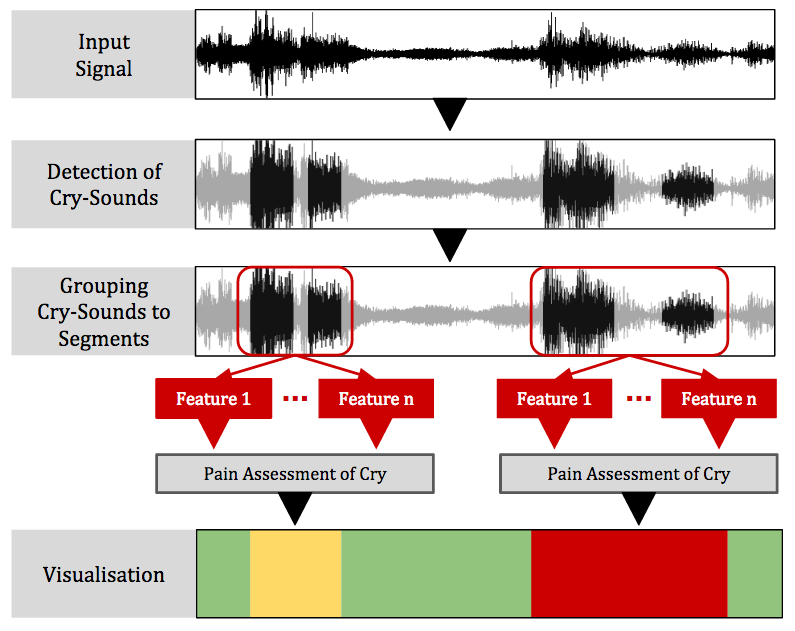
\includegraphics[width=0.9\textwidth]{bilder/konzept04.png}
	\caption{Überblick über die Verarbeitungs-Pipeline}
	\label{img:architecture-overview}
\end{figure}


Der erste Verarbeitungsschritt - die Erkennung der Schreigeräusche - ist notwendig, damit für die Schmerzbewertung des Weinens auch nur solchen Informationen genutzt werden, die tatsächlich vom Weinen eines Babys stammen. Würde man beispielsweise den Schmerzgrad hauptsächlich aus der Tonhöhe des Schreiens ableiten und vorher Störgeräusche wie Hintergrundrauschen nicht als solche erkennen, würden die Tonhöhen dieser Geräusche ebenfalls mit in die Schmerzbewertung einfließen und das Ergebnis verfälschen. Diese Notwendigkeit wurde sowohl von Várallyay \cite{cry_thesis} als auch von Cohen et al. \cite{cohenCry} beschrieben. 

Der zweite Verarbeitungsschritt, die Segmentierung, ist notwendig, da, wie in \autoref{sec:painScores} erläutert, Schmerz-Scores auf Basis der Beobachtung von Zeiträumen bestimmt werden und in einem kontinuierlichen System sinnvolle Anfangs- und Endzeitpunkte für diese Beobachtungszeiträume gefunden werden müssen. Keine der in \autoref{sec:system_literature} vorgestellten Veröffentlichungen präsentiert eine Methode zur Gruppierung der Schreigeräusche, welche für diese Arbeit hätte übernommen werden können. Cohen et al. \cite{cohenCry} schlagen eine feste Segmentlänge von 10 Sekunden vor. Es wurde sich gegen diesen Ansatz entschieden, da die in \autoref{sec:painScores} beschriebenen Schmerz-Scales eine gewisse Flexibilität bezüglich der Beobachtungszeiträume erfordern. In der Dissertation von Várallyay \cite{cry_thesis} ist dieser Verarbeitungsschritt nicht notwendig gewesen, da die Analyse nicht kontinuierlich umgesetzt werden musste und die zu analysierenden Segmente manuell geschnitten wurden. Pal et al. \cite{palEmotion} erwähnen keine Gruppierung von Schreigeräuschen. Aus diesem Grund wurde ein eigener Algorithmus zur Segmentierung entwickelt, welcher in \autoref{sec:segmenting} vorgestellt wird.

Die Berechnung von akustischen Eigenschaften des Weinens und die darauf folgenden Prongnose einer Klasse oder eines Wertes ist ein Verarbeitungschritt, der grundlegend in allen in \autoref{sec:system_literature} vorgestellten Veröffentlichungen angewendet wird. Je nach Ziel der Veröffentlichung werden unterschiedliche Features oder Klassifizierungsmethoden verwendet. Visualisierungskonzepte werden in keiner Veröffentlichung diskutiert, weshalb ein eigener Ansatz entwickelt wurde.

\section{Schmerzbewertung im multimodalen Verbund}
\label{sec:multimodal_integration}

%Schmissiger Begründung
Aus \autoref{sec:pipeline} geht hervor, dass sich die Visualisierung der Schmerzbewertung auf den Score bezieht, der für den Schmerzindikator \emph{Weinen} vergebenen wird. Dies entspricht der Visualisierung eines insgesamten Schmerz-Scores, insofern anstatt einer multimodalen eine unimodale Schmerz-Scale verwendet wird, welche die Schmerzbeurteilung allein anhand des Weinens vornimmt. Ein Beispiel für eine unimodale Schmerz-Scale ist das \glqq Neonatal Facial Coding System\grqq{} (kurz \emph{NFCS}), bei der ein Schmerz-Score ausschließlich anhand der Beobachtung des Schmerzindikators \emph{Gesichtsausdruck} bestimmt wird.\cite[S. 70]{PainAssessment02} Nach Kenntnis des Autors existiert keine unimodale Schmerz-Scale, die sich allein auf das Weinen konzentriert. Es wurde sich dafür entschieden, die Visualisierung allein auf das Scoring des Weinens zu beziehen, damit das Konzept ohne die Miteinbeziehung einer größeren Menge unbekannter Auswertungsergebnisse anderer Schmerzindikatoren erläutert werden kann.

Das vorgestellte Konzept lässt sich zur Visualisierung von Schmerz-Scores in einem multimodalen Verbund erweitern. Dazu wird ein Zwischenschritt vor der Visualisierung eingeführt, bei dem die prognostizierten Scores aller weiteren Schmerzindikatoren zur Score des Weinens über den jeweils selben Diagnosezeitraum addiert werden. Dieses Additionsergebnis - der multimodale Schmerz-Score -  wird daraufhin zur Visualisierung genutzt.

\begin{figure}[h]
	\centering
	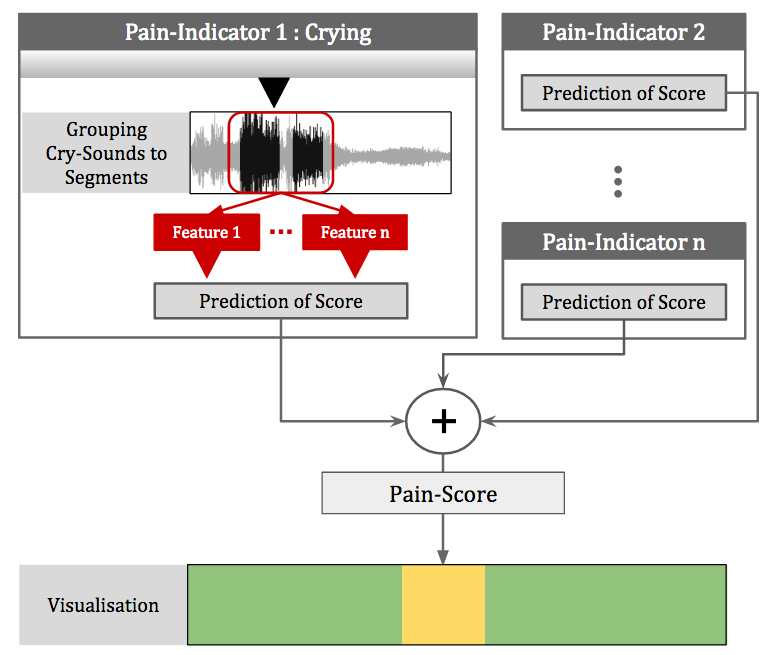
\includegraphics[width=0.7\textwidth]{bilder/multimodal_viz_02.png}
	\caption[Visualisierung im multimodalen Verbund]{Visualisierung im multimodalen Verbund. Oben: Module, welche den Schmerzgrad jeweils eines Indikators in Form eines Scores bewerten. Unten: Visualierung des Schmerz-Scores, welcher durch Addition aller Scores entsteht. }
	\label{img:multimodal-overview}
\end{figure}



